%!TEX root = ../dissertation.tex

\chapter{Explainability in Machine Learning}\label{chapt:explainability}

%TODO Altra possibile roba da aggiungere alla intro, da \cite{samek2019xai}.
%In this match AlphaGo played a move, which was
%classified as “not a human move” by a renowned Go expert, but which was the
%deciding move for AlphaGo to win the game. AlphaGo did not explain the move,
%but the later play unveiled the intention behind its decision. With explainable AI
%it may be possible to also identify such novel patterns and strategies in domains
%like health, drug development or material sciences, moreover, the explanations
%will ideally let us comprehend the reasoning of the system and understand why
%the system has decided e.g. to classify a patient in a specific manner or asso-
%ciate certain properties with a new drug or material. This opens up innumerable
%possibilities for future research and may lead to new scientific insights.

In the last years, thanks to the availability of always larger datasets and due to the always growing computing power of modern GPUs, a lot of artificial intelligence (AI) and deep learning (DL) systems have reached remarkable results in terms of performance on a wide variety of tasks, in some cases largely overcoming human capabilities. Examples are the fields of computer vision, speech recognition or machine translation, which almost always fall into the domain of supervised learning. 
DL, being at the moment the most successful ML approach in supervised learning, has been criticized in \cite{marcus2018appraisal} 
%TODO: aggiungere più references qui... ci sono molti paper che fanno questa critica
for its lack of transparency: in fact, DL systems have millions or even billions of parameters, which are not characterized in human interpretable ways, but only in terms of their position in the network topology. This results in opaque models, to the point that such systems are currently treated almost always as black boxes. DL systems also present other critical issues: in \cite{szegedy2013intriguing} the authors made a neural network misclassify an image by applying an hardly perceptible perturbation, found by maximizing the network’s prediction error. Such adversarial examples have also been found to be somewhat universal and not just the result of overfitting. This poses serious doubts about the ability of NN to learn general representations: indeed, if such networks can generalize well, how can they be confused by nearly indistinguishable images? Similarly, authors in \cite{nguyen2015fooled} show how deep neural networks are easily fooled into misclassifying inputs with no resemblance to the true category. Adversarial examples are not confined to the field of computer vision: natural language networks can also be fooled as shown in \cite{jia2017adversarial}. Furthermore, it has been found that in several applications, DL systems present strong biasedness. One example is reported in \cite{bolukbasi2016debiasing}, where the authors show how word embeddings trained on Google News articles exhibit strong female/male gender stereotypes due to biases in the training data. Susceptibility to unintuitive errors remains therefore a pervasive problem in DL and no robust solution has been found for them so far. Such issues contribute to generate mistrust, and threaten to slow down or even hinder the prevailance of AI in some applications, due to the high potential of unexpected behavior and lack of verifiability of solutions.
%TODO: trovare e inserire altri esempi problematici .... questi potrebbero essere vecchi
In the light of such problems, explainable artificial intelligence (XAI) has become an area of interest in the research community: it tackles the important problem that complex machines and algorithms often cannot provide insights into their behavior and thought processes. The need for XAI is now even more urgent: the renewed EU General Data Protection Regulation (GDPR) could require AI providers to provide users with explanations of the results of ML systems based on their personal data. This clearly affects the industry in a huge way: indeed, the GDPR may hinder or even prohibit the use of \say{black box} models which don't offer explanations for their decisions, when based on users' personal data (think for example to recommender systems). This is also referred to as the \say{right to explanation}. The need for XAI has been also expressed by the statement on algorithmic transparency and accountability released by the Association for Computing Machinery \cite{acm2017transparency}, and by the XAI program launched by DARPA in 2017 \cite{gunning2019xai}.

Even though the general aim for XAI is well understood as the achievement of \textit{interpretability}, or \textit{explainability}, for ML models, few articulate precisely what those terms mean or why they are important. Therefore, the first steps of this chapter will be to define What is explainability, Who needs it, When it is needed and Why.

\section{Why do we need explainability}
\section{When do we need explainability}

\section{What is explainability}
Several research works attempt to describe rigorously the meaning of explainability in the contest of XAI. In the literature, such word is often used interchangeably or substituted by \say{intrepretability}, even though some try to make a distinction. In \cite{gilpin2018explaining}, for example, the authors claim that explainability is a property of a model that implies interpretability, but not viceversa. More specifically, \textit{interpretability} is described as the capability of a certain model to be described in a  way that is understandable to humans; on the other hand, \textit{explainability} is the property of a model to be able to summarize the reasons for their behavior. Explanations, according to the authors, can be evaluated in two ways: according to their \textit{interpretability} (that is, its understandability by a human being) and their \textit{completeness} (that is, the accuracy of the description). Under this definitions, the challenge of XAI is in creating explanations that are both interpretable and complete, even though such characteristics are often opposed to one another. These two features of explanations resemble two important properties of ML models and suggest a similitude: on one hand, the user would desire a simple model with few parameters and at the same time a model able to capture really well the structure of the training data. While both the properties are desirable, they are almost never achievable at the same time. Indeed, as we train simple models, we will probably underfit the data: in the same way, really easy explanations often fail to capture the complexities behind the internal workings of our algorithms. On the other hand, as we add parameters to our model and make it more complex, it will begin to better fit the data: in the same way a really complete explanation will describe accurately the operations of the systems, but will probably result more difficult to understand to a human being. This comparison suggests that, even for explanations, one should allow for a \textit{tradeoff} between interpretability and completeness. The author suggests also that the explanation methods should be evaluated according to how such explanations behave on the curve from maximum interpretability to maximum completeness. Figure \ref{fig:example_explainability} gives a visualzation of this concept.

\begin{figure}
	\centering
	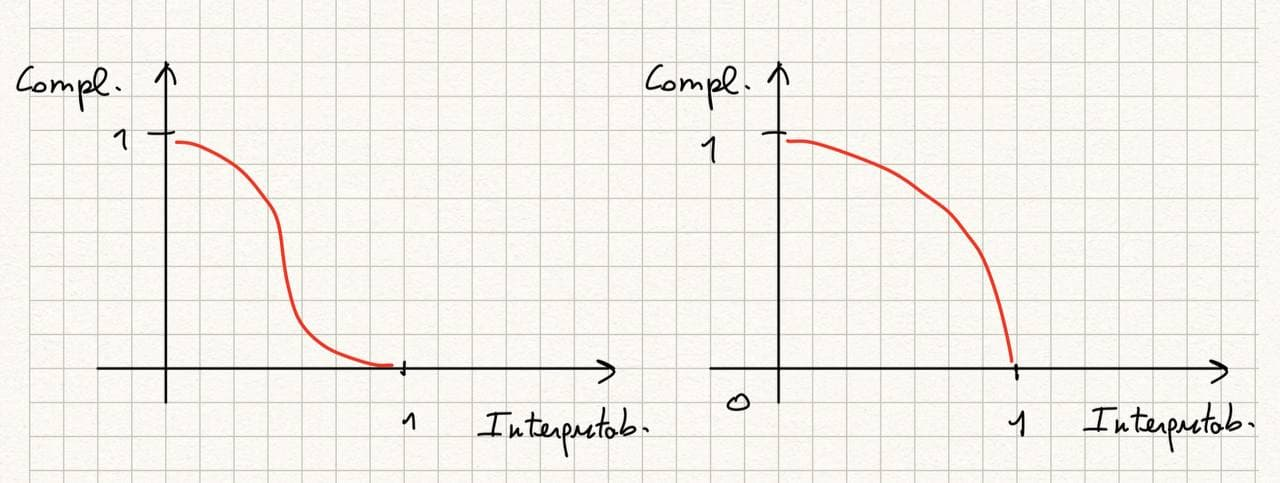
\includegraphics[width=0.9\linewidth]{figures/example_explainability.png}
	\caption{Example of two different explanations according to the definition given by \cite{gilpin2018explaining}: each explanation allows for a tradeoff between completeness and interpretability. Explanation on the right should be evaluated better than the one on the left: indeed, for higher values of interpretability, the right one offers higher values of completeness.}
	\label{fig:example_explainability}
\end{figure}

In \cite{doshivelez2017rigorous} interpretability is defined as the ability to explain or to present in understandable terms to a human. According to \cite{burkart2021survey}, instead, \textit{interpretability} is most often used in terms of comprehending how the prediction model works as a whole, while \textit{explainability}, in contrast, is used to indicate the capability of models to give explanations about their decision, but keeping their black box nature. In the particular context of generating explanations for DL models, the authors of \cite{montavon2018methods} define an explanation as the collection of features of an interpretable domain (i.e. pixel values on images), that have contributed for a given example to produce a decision (e.g. classification or regression). We can see that none of the aforementioned definitions are specific enough to enable one universal formalization: indeed they implicitly  depend on the context or the aim of the research work. We will now try to give definitions that better summarize the mentioned ones.

\begin{definition}[Interpretability]
	\label{def:interpretability}
	We define \textit{interpretability} in the context of supervised ML as the generic property of a model which makes its single components, as well as its functioning as a whole, understandable by a human being. Examples of interpretable models are simple linear regression or decision trees. Examples of not interpretable models are deep neural networks.
\end{definition}

\begin{definition}[Explainability]
	\label{def:explainability}
	We define \textit{explainability} in the context of supervised ML as the generic property of a model which makes it able to explain, to a certain extent, its own reasons behind a certain decision.
\end{definition}

In general, it is true that an explainable model is almost always interpretable, but the viceversa might not always be true. An exception to this rule, however, even if outside the field of ML, is the human brain: while we are able to give really detailed and motivated reasons behind our decision processes, our brain is not an interpretable model. Indeed, we don't know every single aspect of how our brains works, and yet we (often) trust the explanations that other human beings provide when asked why they took a certain decision. This offers an interesting point of view to the discussion: we should be careful not to trust certain explanations only by the fact that they look plausible and convincing. To this regard, Herman \cite{Herman2017ThePA} warns us, making a clear distinction between descriptive and persuasive explanations: indeed implicit cognitive biases of the human brain could threaten transparency (for example, humans naturally tend to prefer simpler descriptions). To avoid falling in this problem, one should always keep in mind the tradeoff process between completeness and interpretability, mentioned above.

Even after an attempt of definitions, the meaning of interpretability, and explainability is still too generic and can be applied to any ML model. In fact, the volume of research in interpretability is quickly expanding, making the number of available methodologies continuously grow. Despite that, two main categories of approaches to interpretability and explainability are often distinguished \cite{dosilovic2018explainable, lipton2017mythos}: integrated interpretability, or \textit{transparency} and \textit{post-hoc} interpretability.

\subsection{Transparency}

Transparency is one of the properties that can enable interpretability and it implies some sort of understanding of the mechanism by which the model works. It can also be seen as the direct opposite to the concept of \textit{black box}. Lipton \cite{lipton2017mythos} goes into even more details, by subdividing transparency in different levels:
\begin{enumerate}
	\item \textbf{Simulatability}: it's the highest level of abstraction of the concept of transparency. Lipton refers to simulatability as the property of the model that makes it understandable by a person \say{at once}. Specifically, this means that a human could, given the input data and all the necessary parameters, produce a prediction by making all the computations in a reasonable time. 
	\item \textbf{Decomposability}: it's the transparency considered at the level of the single components of the model. Specifically, one model can be considered decomposable if each part of the model (weights, modules, computations...) admits an intuitive explanation.
	\item \textbf{Algorithmic Transparency}: this notion transparency refers to the learning algorithm itself. For example, we know that in the case of linear regression the shape of the loss function is known, as well as an analytical form for the solution for the problem. This means a maximum degree of algorithmic transparency. On the other hand, modern deep learning lacks this notion of transparency: in fact, even if a lot of powerful optimization algorithms give empirically excellent results, there is no guarantee that those will work on any new problem. The same holds for the shape of the error function, which is almost never known.
\end{enumerate}

It's interesting to notice that the human brain, as noted previously, doesn't exhibit any of those features. In fact, human thinking is not transparent to us and justifications in the form of explanations may differ from the actual decision mechanism.

\subsection{Post-hoc interpretations}

%TODO now refine this part...

Post hoc interpretability extracts informations from already learned models and it does not precisely depend on how the model works. the advantage of this approach is that it does not impact performance of the model, which is treated as a black box. special care in order to not generate plausible but misleading explanations.(riferimento a articolo Herman, he notes that we should be wary of evaluating interpretable systems using merely huuman evaluations of interpretability, because human evaluations imply a strong and specific bias towards simpler descriptions)
(trovare il modo di parlare di activation maximization... global vs local..., poi ricordarsi di attaccare il discorso difficoltà di integrare prior knowledge)



%Lipton paper: \cite{lipton2017mythos}.
%Methods for interpreting and understanding... \cite{MONTAVON20181}.
%Explaining Explanations... \cite{gilpin2018explaining}
%Explainable artificial Intelligence: a survey \cite{dosilovic2018explainable}
%Towards a rigorous science... \cite{doshivelez2017rigorous}
%kenn paper: \cite{daniele2019kenn}
%survey on the explainability of supervised ml \cite{burkart2021survey}.
%test article: \cite{article1}



